\chapter{Hardware Arkitektur}

\subsection{Block Definition Diagram}

\begin{figure}[H]
	\centering
	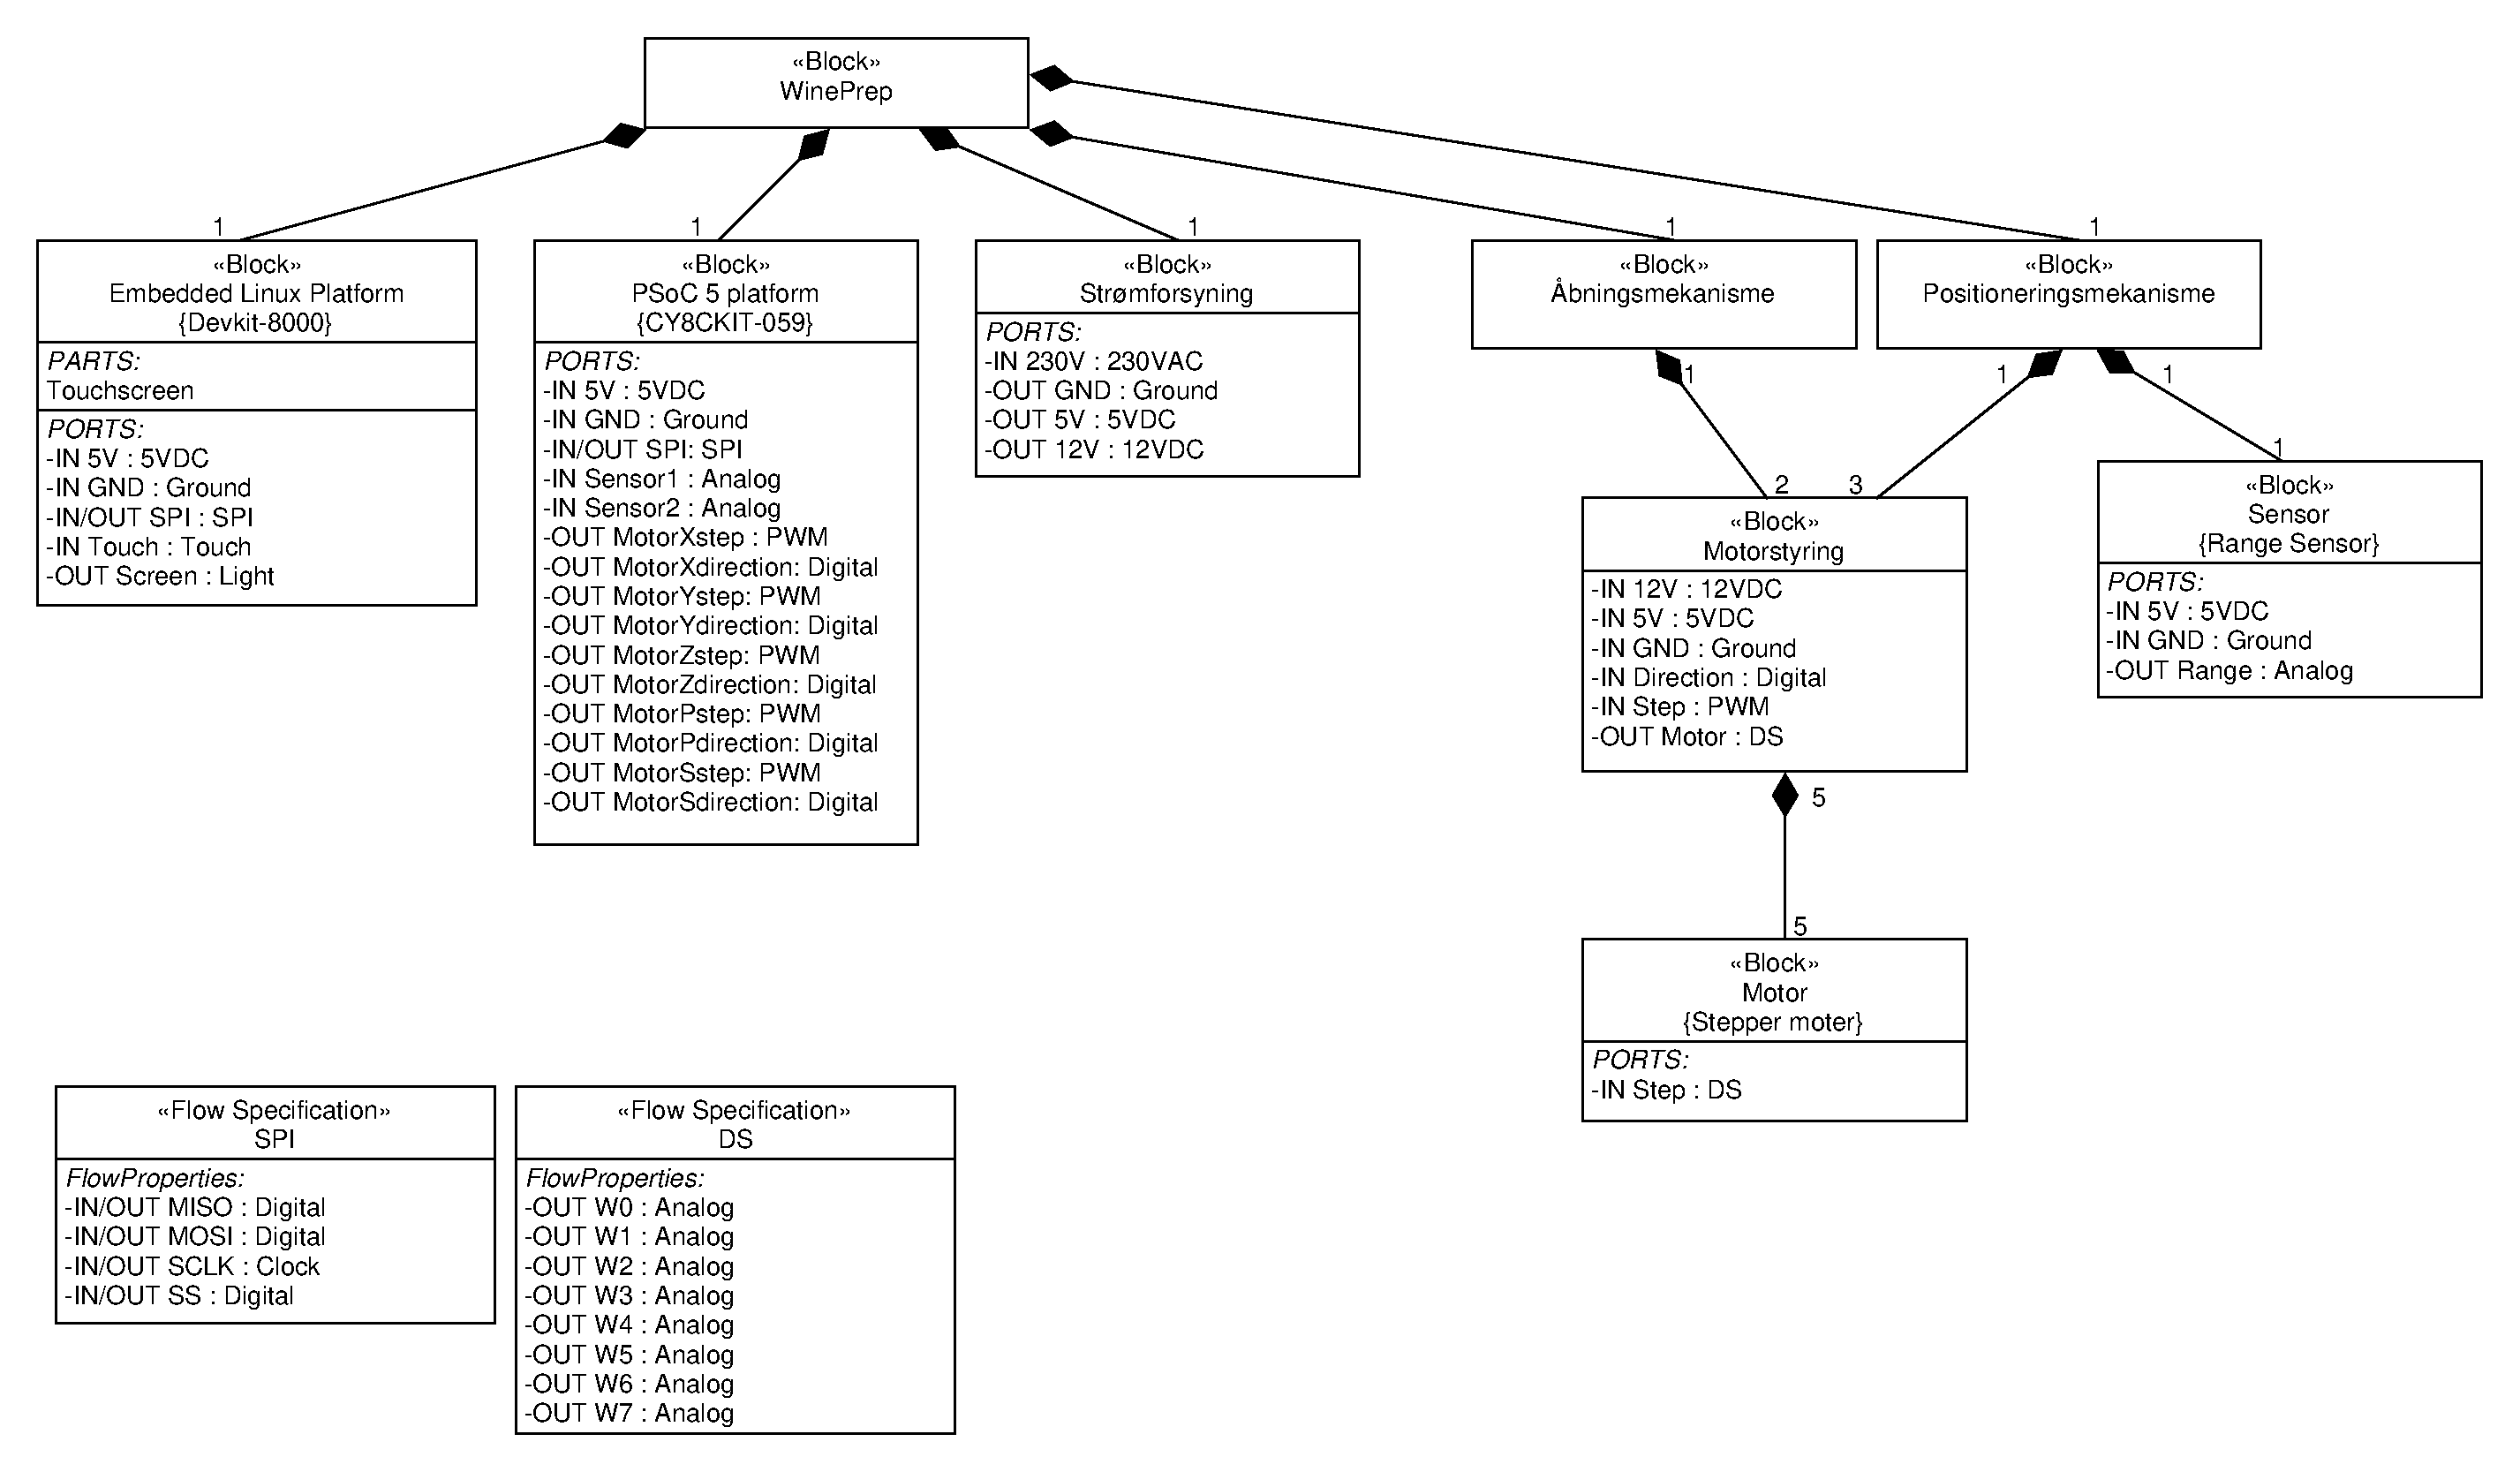
\includegraphics[scale=0.3]{blockdefinitiondiagram}
	\caption{BDD for WinePrep}
	\label{BDD}
\end{figure}

\subsubsection{Blok beskrivelser}
Her følger beskrivelser af de enkelte blokke på vores BDD, se side \pageref{BDD} Figur \ref{BDD}.

\paragraph{WinePrep} blokken er det samlede system der består af underblokkende Embedded Linux Platform, PSoC 5 Platform samt Åbningsmekanismen.

\paragraph{Embedded Linux Platform} Dette er den blok der håndtere brugerens interaktion med systemet. Blokken består af et Devkit800 med touchskærm. Som styresystem på platformen anvendes der Linux distributionen Ångström. Her fra anvendes der QT til at lave den grafiske brugerflade der vises på touchskærmen til brugeren af systemet. Samtidig kommunikere Embedded Linux Platformen med vores PSoC 5 Platform via SPI standarden.

\paragraph{PSoC 5 Platform} PSoC 5 baseret platform der står for styring af Motor og Sensor blokkene, samt kommunikere med blokken Embedded Linux Platform over SPI.

\paragraph{Motor} Denne blok definere de aktuatore der anvendes til at trække proppen op af vinen samt til at sikre at åbningsmekanismen rammer vinflasken korrekt uden at vælge eller beskadige vinen.

\paragraph{Sensor} Afstandssensorer til detektering af vinflaskens placering samt størrelse, så åbningsmekanismen ud fra dette kan positioneres korrekt ved hjælp af motorer på X, Y , Z akserne.

\subsection{Ting der først bliver fast besluttet på senere iterationer/sprints}

Motor Valg er ikke 100\% fastlagt, hvorfor det her i BDD modelleres med stepper motors, og portene er derfor heller ikke 100\% korrekte da dette afhænger af motorstyringen.

Sensor typer og antal ligger kun delvist fast, der vil være minimum 2 afstandssensorer af en art, hvorfor BDD er lavet mod 2 sensorer, det bliver enten lys baserede eller lydbaserede, der vil give et analog output signal i form af en spænding der afhænger af afstanden.